\chapter{Analisi dei requisiti}
Un sistema informatico deve, in genere, risolvere un determinato problema relativo ad una categoria di utenza. Per raggiungere l'obiettivo deve quindi fornire un certo numero di funzionalità relative alla gestione delle informazioni, possedendo caratteristiche precise di efficienza e affidabilità. I requisiti riguardano per l'appunto la comprensione e la descrizione del problema da risolvere mediante l'implementazione di funzionalità e di qualità desiderate per il sistema.
\section{Stakeholders}
Si definisce \textit{stakeholder} una qualsiasi entità dotata di comportamento che interagisce con il sistema informatico in questione. Quest'ultimo è inoltre considerato anch'esso uno stakeholder quando interagisce con altri sistemi informatici, nel caso del progetto Garzone  quando interagisce, ad esempio, con il sistema di pagamento adottato.
\subsection{Attori primari}
Un'entità che utilizza direttamente la soluzione per perseguire i suoi obiettivi è considerata un attore primario. In Garzone gli attori primari sono rappresentati da:
\paragraph{Negozi} Entità costituite da un punto vendita fisico in un determinato comune registrato sulla piattaforma. Sono rappresentati da un titolare o referente che ha il compito di gestire il proprio catalogo e interagire con i clienti finali utilizzando le varie funzionalità
\paragraph{Comuni} Organi della pubblica amministrazione che delegano un funzionario facente parte della giunta eletta per la gestione e il controllo dei negozi registrati alla piattaforma. Il loro ruolo è meramente di supervisione, possono infatti abilitare o disabilitare la visualizzazione di negozi nel marketplace. Inoltre hanno la possibilità di scambiare comunicati con i negozi.
\paragraph{Amministratore} Persona o gruppo di persone organizzate per la gestione e la supervisione complessiva della piattaforma. L'amministrazione avviene mediante l'interazione con negozi, comuni e clienti che necessitano di supporto o di interventi particolari, come la disabilitazione per condotte scorrette. In Garzone questa mansione è per ora affidata all'azienda stessa, ma in futuro è prevista una delegazione a terzi.
\subsection{Attori finali}
Sono definiti attori finali coloro che usufruiscono del servizio messo a disposizione per raggiungere i propri obiettivi. In Garzone è previsto un solo attore finale: il cliente.
\paragraph{Cliente}
I clienti rappresentano il bacino di utenza della piattaforma e hanno la possibilità di interagire con i negozi per raggiungere i propri obiettivi, quali l'acquisto di beni/servizi, la comunicazione diretta con i corrispondenti referenti, la richiesta di preventivi, la prenotazione di appuntamenti, la visualizzazione dei cataloghi e altro.
\subsection{Attori di supporto}
Generalmente gli attori di supporto offrono alla soluzione servizi esterni necessari per il suo corretto funzionamento. Spesso sono sistemi informatici, ma possono anche essere rappresentati da società/organizzazioni o persone fisiche
\paragraph{Servizio di autorizzazione dei pagamenti} In Garzone è prevista un'interfaccia ad un servizio di autorizzazione dei pagamenti per autorizzare i pagamenti correttamente ed evitare tentativi di frode. Inoltre ha il compito di registrare le transazioni dirette tra Clienti e Negozi.
\paragraph{Servizio di autenticazione degli utenti} Per la corretta gestione degli utenti e la prevenzione di attacchi informatici sui dati di registrazione, Garzone si interfaccia a un servizio esterno di registrazione e autenticazione degli utenti. Esso ha il compito di comunicare con il sistema informatico e garantire il corretto flusso di registrazione, accesso e gestione delle utenze.
\paragraph{Servizio di geolocalizzazione} Per offrire un'esperienza utente migliore, in Garzone è prevista l'implementazione di un'interfaccia ad un servizio di geolocalizzazione, il quale ha il compito di interpretare indirizzi geografici forniti dal sistema e restituire delle coordinate geografiche precise.
\section{Requisiti}
Un requisito è una capacità o una condizione a cui il sistema, e più in generale, il progetto, deve essere conforme\cite{JBR99}. La modellazione dei requisiti avviene secondo le necessità degli utenti del sistema per risolvere le proprie problematiche.
\subsection{Requisiti funzionali e non funzionali}
I requisiti funzionali riguardano, attraverso l'implementazione delle varie funzionalità, il comportamento del sistema informatico nel suo complesso. Tra i requisiti funzionali rientrano anche i casi d'uso.
Vengono definiti invece requisiti non funzionali tutti i requisiti che non sono determinanti nel funzionamento della soluzione informatica (Garzone), ma sono relativi alle sue proprietà nel suo complesso, come ad esempio prestazioni, scalabilità, usalibilità e prestazioni.

\section{Casi d'uso}
Un caso d'uso, seguendo le linee guida RUP (Rational Unified Process), è un insieme di istanze di casi d'uso, in cui ciascuna istanza è una sequenza di azioni che un sistema esegue per produrre un risultato osservabile e di valore per uno specifico attore\cite{RUP}. Per convenzione, i casi d'uso che prevedono la parola chiave "gestisci" riuniscono gli obiettivi separati CRUD (create, retrieve, update, delete) in un unico caso CRUD.
\subsection{Casi d'uso in Garzone}
I casi d'uso possono essere descritti, in genere, in diversi modi. Per la definizione dei casi d'uso relativi a Garzone, si è optato per una stesura in formato breve, ovvero riepiloghi brevi e precisi relativi ai soli scenari di successo. Di seguito vengono elencati i principali casi d'uso.
\paragraph{Registra Negozio} Il negozio, tramite il suo titolare o l'addetto all'utilizzo della piattaforma, compila manualmente i dati relativi alla sua registrazione. Il sistema, dopo la convalida dei dati e mediante l'interfaccia con il servizio di autenticazione degli utenti e di geolocalizzazione, registra l'utenza.
\paragraph{Registra Cliente} Il cliente compila manualmente i dati relativi alla sua registrazione. Il sistema, dopo la convalida dei dati e mediante l'interfaccia con il servizio di autenticazione degli utenti e di geolocalizzazione, registra l'utenza.
\paragraph{Gestisci Vetrina} Il negozio, tramite il suo titolare o l'addetto all'utilizzo della piattaforma, aggiunge o modifica prodotti e servizi del suo catalogo. L'utente in questione inserisce manualmente i dettagli del prodotto o servizio. Il sistema convalida i dati e registra l'inserimento o la modifica. I clienti saranno in grado di navigare sulla vetrina del negozio e visionarne il catalogo.
\paragraph{Gestisci Promozione} Il negozio, tramite il suo titolare o l'addetto all'utilizzo della piattaforma, aggiunge una promozione relativa a un prodotto/servizio offerto. L'utente in questione inserisce manualmente i dati relativi alla promozione tra cui la data di scadenza. Il sistema convalida e registra la promozione. I clienti saranno in grado di visionare solo le promozioni attive del negozio ed eventualmente usufruirne.
\paragraph{Gestisci Appuntamento} Il negozio, tramite il suo titolare o l'addetto all'utilizzo della piattaforma, crea un evento per un determinato orario referenziando un cliente coinvolto. L'addetto che registra l'appuntamento inserisce i dati manualmente e, dopo convalida e registrazione, il sistema notifica il cliente della creazione dell'evento.
\paragraph{Crea Ordine} Il cliente, dopo essersi autenticato, dalla pagina di vetrina del negozio aggiunge prodotti messi a disposizione dal negozio al carrello. Il sistema dopo averne calcolato il totale richiede al cliente, tramite interfaccia grafica, l'inserimento manuale di dati relativi all'evasione dell'ordine. Nel caso in cui il cliente volesse che il suo ordine sia evaso ritirandolo in negozio non sarà necessario specificare un indirizzo di consegna, viceversa dovrà essere inserito. Il sistema, dopo la conferma da parte del cliente, registra l'ordine e il negozio viene notificato dell'avvenuta creazione.
\paragraph{Accetta Ordine} Il negozio, tramite il suo titolare o l'addetto all'utilizzo della piattaforma, accetta la richiesta di ordine effettuata dal cliente. Dopo l'accettazione dell'ordine, il negozio procede con la sua evasione, specificando per gli ordini di consegna a domicilio un eventuale costo di consegna. Il sistema registra il cambio di stato dell'ordine. Il cliente dopo la modifica viene notificato automaticamente dell'avvenuto aggiornamento e del totale aggiornato, comprensivo del costo di consegna inserito.
\paragraph{Paga Ordine} Il cliente, dopo l'autenticazione e dopo l'approvazione dell'ordine che prevede un pagamento online da parte del negozio e l'eventuale inserimento del costo di consegna per gli ordini di consegna a domicilio, procede con il pagamento online. Il sistema calcola il totale dell'ordine comprensivo del costo di consegna e delega al sistema di autorizzazione dei pagamenti il completamento dell'operazione. Il sistema notifica il negozio e il cliente dell'avvenuto pagamento e aggiorna lo stato attuale dell'ordine.
\paragraph{Evadi Ordine} Il negozio, tramite il suo titolare o l'addetto all'utilizzo della piattaforma, modifica lo stato dell'ordine. Per gli ordini con pagamento online il negozio procede con l'effettiva consegna e il cambio di stato dell'ordine. Per gli ordini che prevedono il ritiro in negozio, la preparazione dei prodotti/servizi richiesti per il ritiro e il successivo cambio di stato dell'ordine. Il sistema registra il cambio di stato dell'ordine e notifica il cliente.
\paragraph{Invia Preventivo} Il negozio, tramite il suo titolare o l'addetto all'utilizzo della piattaforma, inserisce manualmente i dati relativi a un preventivo. Il sistema, dopo aver convalidato i dati inseriti, invia il preventivo contenente i dettagli di un possibile ordine al cliente. Il cliente accetta il preventivo e il sistema aggiorna lo stato dell'ordine notificando il negozio dell'avvenuto aggiornamento.
\paragraph{Accetta Preventivo} Il cliente, dopo la sua autenticazione e la ricezione di un preventivo da parte del negozio, accetta la proposta. Il sistema aggiorna lo stato dell'ordine e notifica il negozio dell'avvenuto cambiamento.
\paragraph{Invia Messaggio} Il cliente, dopo la sua autenticazione, avvia una conversazione di chat con il negozio (o viceversa). Dopo la validazione del messaggio, il sistema provvede alla sua registrazione. Il negozio (il cliente) viene notificato della sua ricezione e viene abilitato ad inviare a sua volta un messaggio.
\paragraph{Abilita Negozio} Il comune, dopo la sua autenticazione, abilita o disabilita un negozio, rendendone impossibile l'accesso e la visualizzazione sulla piattaforma.
\paragraph{Gestisci Comunicazione} Il comune, dopo la sua autenticazione, aggiunge una comunicazione, la quale sarà visibile ai negozianti e agli utenti del marketplace.
\paragraph{Gestisci Comune} L'amministratore di sistema, dopo la sua autenticazione, provvede a gestire i dati relativi ad un comune. Dopo la compilazione manuale dei dati del comune, il sistema li convalida e registra/aggiorna l'istanza. 
\paragraph{Gestisci Negozio} L'amministratore di sistema, dopo la sua autenticazione, provvede a gestire i dati relativi ad un negozio. Dopo la compilazione manuale dei dati del negozio, il sistema li convalida e registra/aggiorna l'istanza. 
\paragraph{Gestisci Cliente} L'amministratore di sistema, dopo la sua autenticazione, provvede a gestire i dati relativi ad un cliente. Dopo la compilazione manuale dei dati del cliente, il sistema li convalida e registra/aggiorna l'istanza.

\begin{table}[!htb]
    \centering
    \begin{tabular}{|c|c|} 
    \hline
    \textbf{Caso d'uso}             & \textbf{Attori coinvolti}                         \\ 
    \hline
    \textit{Registra Negozio}       & Negozio, Amministratore, Servizio autenticazione, \\ &Servizio di geolocalizzazione  \\ 
    \hline
    \textit{Registra Cliente}       & Cliente, Servizio autenticazione, \\ & Servizio di geolocalizzazione                  \\ 
    \hline
    \textit{Gestisci Vetrina}       & Negozio, Amministratore                           \\ 
    \hline
    \textit{Gestisci Promozione}    & Negozio, Amministratore                           \\ 
    \hline
    \textit{Gestisci Appuntamento}  & Negozio, Cliente, Amministratore                  \\ 
    \hline
    \textit{Crea~Ordine}            & Cliente                                           \\ 
    \hline
    \textit{Accetta Ordine}         & Negozio, Amministratore                           \\ 
    \hline
    \textit{Paga Ordine}            & Cliente, Servizio autorizzazione pagamenti        \\ 
    \hline
    \textit{Evadi Ordine}           & Negozio, Amministratore                           \\ 
    \hline
    \textit{Invia Preventivo}       & Negozio                                           \\ 
    \hline
    \textit{Accetta Preventivo}     & Cliente                                           \\ 
    \hline
    \textit{Invia Messaggio}        & Negozio, Cliente                                  \\ 
    \hline
    \textit{Abilita Negozio}        & Comune, Amministratore                            \\ 
    \hline
    \textit{Gestisci Comune}        & Comune,~Amministratore, Servizio autenticazione,\\ & Servizio di geolocalizzazione                            \\ 
    \hline
    \textit{Gestisci Negozio}       & Negozio,~Amministratore, Servizio autenticazione,\\ & Servizio di geolocalizzazione                           \\ 
    \hline
    \textit{Gestisci Cliente}       & Cliente, Amministratore, Servizio autenticazione, \\ &Servizio di geolocalizzazione                           \\ 
    \hline
    \textit{Gestisci Comunicazione} & Comune, Amministratore                            \\
    \hline
    \end{tabular}
    \caption{Riepilogo Casi d'uso e Attori coinvolti}
\end{table}

\section{Modellazione astratta e struttura del progetto}
Garzone ha lo scopo di rendere possibile la transizione vera e propria di un negozio fisico al digitale fornendo ai negozianti una piattaforma gestionale efficiente e ai cittadini un efficacie canale di comunicazione. Per ogni attore è prevista la realizzazione di una propria piattaforma con un dominio web dedicato. \\Tutte le piattaforme comunicano per la gestione dati con un sistema backend unico, il quale a sua volta si interfaccia con sistemi per l'autorizzazione dei pagamenti, per l'autenticazione degli utenti e una base di dati.
\subsection{Pannello Negozio}
Il pannello del negoziante prevede l'implementazione delle seguenti funzionalità:
\begin{itemize}
    \item \textbf{Registrazione}: consiste in una sezione dove viene richiesto al negoziante di registrarsi, selezionando prima il marketplace (comune) in cui è ubicato e poi inserendo manualmente sia dati personali che dati fiscali relativi al negozio fisico
    \item \textbf{Accesso}: prevede una sezione dove un negozio registrato effettua l'accesso previa una registrazione già effettuata e l'effettiva abilitazione da parte del comune
    \item \textbf{Dashboard}: contiene una data visualization tramite grafici dei dati più rilevanti riguardo la gestione del negozio
    \item \textbf{Gestione dati relativi all'utenza registrata}: prevede una sezione in cui è possibile per il negoziante modificare dati fiscali relativi al negozio o dati personali
    \item \textbf{Gestione funzionalità attive}: offre la possibilità al negoziante di abilitare/disabilitare funzionalità di Garzone relative al suo negozio, come ad esempio i pagamenti online
    \item \textbf{Gestione prodotti/servizi}: da questa sezione è possibile gestire mediante creazione, modifica ed eliminazione tutti i prodotti/servizi presenti nel catalogo del negozio fisico
    \item \textbf{Gestione promozioni}: da questa sezione è possibile inserire, modificare ed eliminare promozioni
    \item \textbf{Gestione appuntamenti}: da questa sezione è possibile inserire, modificare ed eliminare appuntamenti
    \item \textbf{Gestione ordini}: da questa sezione è possibile gestire gli ordini ricevuti dai clienti, i quali seguiranno un flusso di evasione prestabilito
    \item \textbf{Invio messaggi}: tramite questa sezione il negoziante potrà comunicare solo con clienti hanno precedentemente inviato un messaggio al negozio
    \item \textbf{Visualizzazione comunicazioni}: contiene le comunicazioni create dal comune in cui il negozio è registrato
\end{itemize}
\subsection{Pannello Comune} Il pannello del comune prevede l'implementazione delle seguenti funzionalità:
\begin{itemize}
    \item \textbf{Accesso}: prevede una sezione dove un comune registrato effettua l'accesso, previa una registrazione già effettuata dall'amministratore di Garzone e l'effettiva abilitazione
    \item \textbf{Dashboard}: contiene una data visualization tramite grafici dei dati più rilevanti riguardo la gestione del negozio
    \item \textbf{Gestione dati relativi all'utenza registrata}: prevede una sezione in cui è possibile per il comune modificare dati fiscali relativi all'organo amminsitrativo e dati relativi al suo referente
    \item \textbf{Abiltazione negozi}: da questa sezione è possibile abilitare o disabilitare i negozi del proprio comune (marketplace)
    \item \textbf{Gestione comunicazioni}: tramite questa sezione il comune potrà comunicare ai negozianti del proprio marketplace avvisi rilevanti
\end{itemize}
\subsection{Pannello Amministratore} Il pannello di amministrazione prevede l'implementazione delle seguenti funzionalità:
\begin{itemize}
    \item \textbf{Accesso}: prevede una sezione dove l'amministratore può accedere alla sua piattaforma
    \item \textbf{Dashboard}: contiene una data visualization tramite grafici dei dati più rilevanti riguardo negozi, comuni e clienti
    \item \textbf{Gestione comuni}: tramite questa sezione l'amministratore può gestire, inserendo, modificando o eliminando, i dati dei comuni
    \item \textbf{Gestione negozi}: da questa sezione è possibile gestire tramite inserimento, modifica ed eliminazione, i dati fiscali, i dati relativi al negozio fisico, le chat, gli ordini e gli appuntamenti dei negozianti nei vari marketplaces
    \item \textbf{Gestione clienti}: tramite questa sezione l'amministratore può gestire, inserendo, modificando o eliminando, i dati dei clienti e relativi ordini, chat e appuntamenti
    \item \textbf{Gestione promozioni}: tramite questa sezione l'amministratore può gestire, inserendo, modificando o eliminando, i dati delle promozioni create dai negozianti
\end{itemize}
\subsection{Pannello Cliente} Il pannello destinato ai clienti, invece prevede lo sviluppo delle seguenti funzionalità:
\begin{itemize}
    \item \textbf{Registrazione}: consiste in una sezione dove viene richiesto al cliente di registrarsi, inserendo manualmente i suoi dati personali
    \item \textbf{Accesso}: prevede una sezione dove il cliente può accedere alla piattaforma di Garzone
    \item \textbf{Visualizzazione marketplace}: prevede la possibilità per il cliente di visualizzare tutti i negozi, registrati e abilitati dalla piattaforma, di un comune da lui selezionato
    \item \textbf{Visualizzazione promozioni}: revede la possibilità per il cliente di visualizzare tutte le promozioni inserite dai negozi  e attualmente attive (non scadute) per il marketplace selezionato
    \item \textbf{Visualizzazione negozio}: prevede la possibilità per il cliente di visualizzare i dettagli di registrazione, il catalogo prodotti/servizi con la possibilità di aggiunta al carrello per un successivo ordine, le promozioni e gli slot di appuntamento già occupati di un negozio specifico selezionato dal marketplace
    \item \textbf{Invio messaggi}: tramite questa sezione il cliente, previa registrazione e accesso, ha la possibilità di inviare messaggi ad un negozio selezionato
    \item \textbf{Richiesta preventivo}: tramite questa funzionalità un cliente può richiedere un preventivo al negoziante indicando le sue necessità
    \item \textbf{Gestione ordini}: da questa sezione è possibile gestire gli ordini inviati ai negozi, i quali seguiranno un flusso di evasione prestabilito
    \item \textbf{Gestione appuntamenti}: da questa sezione è possibile gestire, modificando o annullando, gli appuntamenti presi con i negozi dei vari marketplaces
    \item \textbf{Visualizzazione comunicazioni}: contiene le comunicazioni create dal comune (marketplace) selezionato
\end{itemize}
\newpage
I domini della soluzione costituiscono una struttura gerarchica ad albero, in cui il pannello cliente è consultabile tramite dominio principale, mentre gli altri pannelli tramite sottodomini. L'idea generale segue questa struttura:
\begin{figure}[!htb]
    \centering
    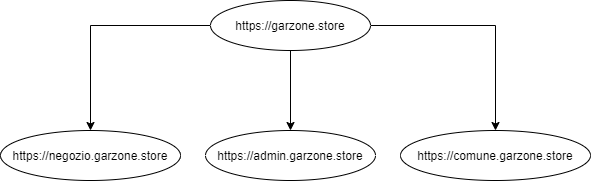
\includegraphics[width=0.8\textwidth]{domini.png}
    \caption{Struttura domini e sottodomini Garzone}
\end{figure}
\\
Le varie piattaforme comunicano tra loro interfacciandosi al servizio di autenticazione delle utenze e ad un sistema backend condiviso, il quale a sua volta si interfaccia a un'apposita base di dati e al servizio di autorizzazione dei pagamenti.
\begin{figure}[!htb]
    \centering
    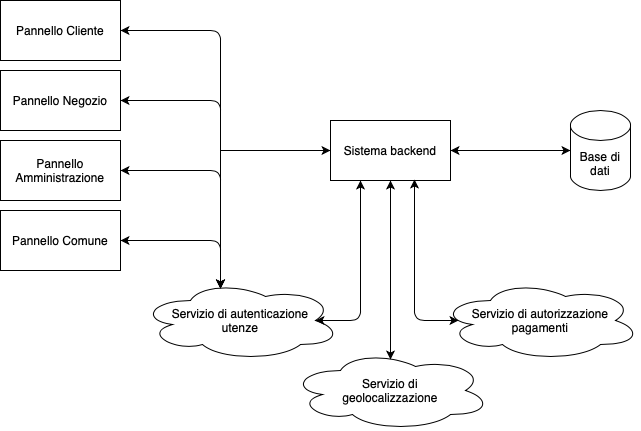
\includegraphics[width=1\textwidth]{modelloastratto.png}
    \caption{Modello complessivo astratto di implementazione}
\end{figure}
\\